% \includemedia[
%   addresource=files/ski_mask_v2.mp3,    % Name of the audio file
%   flashvars={
%     source=files/ski_mask_v2.mp3,        % Again specify the source
%     &autoPlay=false            % Automatically starts playing on slide open
%   },
%   transparent,
%   passcontext  % passes clicks to FlashPlayer
% ]{\fbox{Play}}{VPlayer.swf}
% Vision transformer, LLM (sequence), tokenization for time series.

\begin{frame}{Transformer basics}

\begin{itemize}
    \item Transformers are a type of feedforward neural network distinguished by the presence of {\it transformer blocks}
    \item The original paper by \citet{Vaswani2017-em} has over 120,000 citations
    \item We'll focus on sequence-to-sequence transformers
\end{itemize}
\begin{align*}
    &T: \mathcal H^L \to \mathcal H^L \\
    &\text{$L :=$ input sequence length, $\mathcal H :=$ set of tokens}
\end{align*}
\begin{figure}
    \centering
    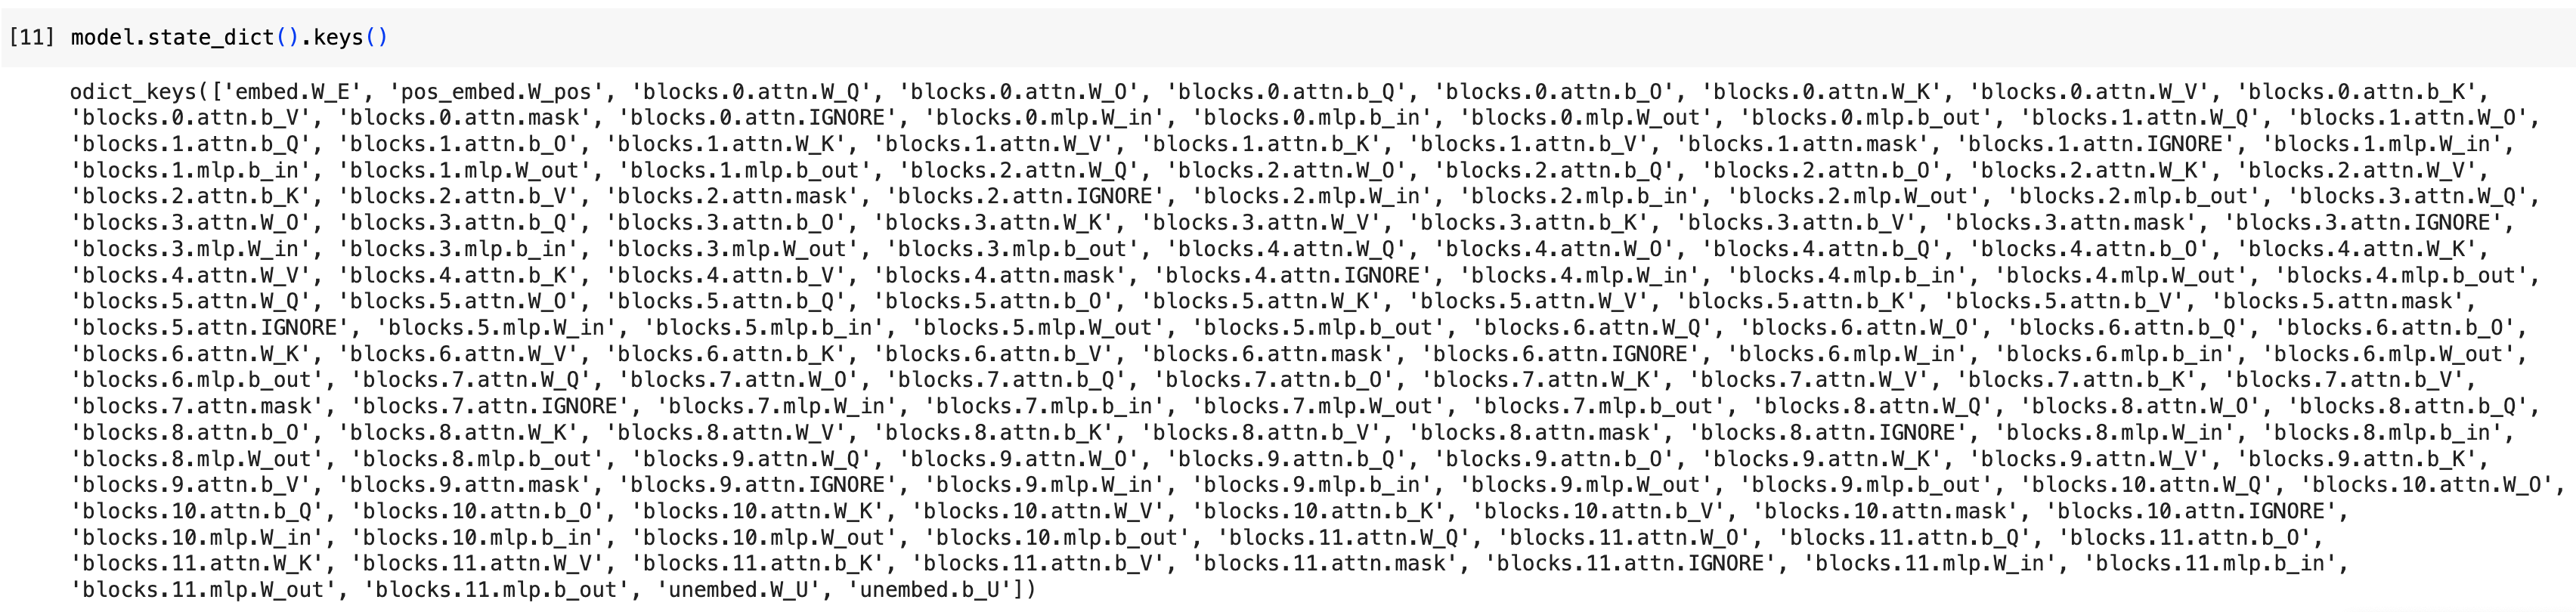
\includegraphics[width=12cm]{img/gpt2keys.png}
    \caption*{GPT2-small model parameter groups (number of blocks $B = 12$)}
    \label{fig:enter-label}
\end{figure}
\end{frame}

\begin{frame}{Transformer basics}
\begin{itemize}
    \item Start with a random embedding $T_{*} : \mathcal H \to \mathbb R^m$
    \item Blocks $T_b : \mathbb R^{m \times L} \to \mathbb R^{m \times L}$ progressively deform projection of tokens into $\mathbb R^{m \times L}$
    \item An unembedding $T_{-*}: \mathbb R^m \to \mathbb R^{|\mathcal H|}$ followed by softmax $s : \mathbb R^{|\mathcal H|} \to \mathbb R^{|\mathcal H|}$ is applied after the last block
    \begin{align}
        T(h_L) = s^L \circ T_{-*}^L \circ T_{B-1} \circ T_{B-2} \circ \dotsc \circ T_0 \circ T_* (h_L)
    \end{align}
    \item During training, target variables are shifted right by one version of input variables, and a mask is used on the {\it attention mechanism} so that the network only has knowledge of previous positions in the sequence
    \item During inference, last position in sequence is appended over repeated forward passes
\end{itemize}
\end{frame}

%x &\mapsto \frac{e^{x_l}}{\sum_{l \in [L]} e^{x_l}} \\ 
\begin{frame}{Transformer blocks}
\begin{columns}
\begin{column}{.5\textwidth}
\begin{itemize}
    \item Each block consists of an attention mechanism $A_b$ and {\it multilayer perceptron} $M_b$
\begin{align*}
    T_b = M_b^L \circ A_b % why do these and also the flow networks have a two part structure?
\end{align*}
    \item $A_b: \mathbb R^{m \times L} \to \mathbb R^{m \times L}$
    \item $M_b: \mathbb R^m \to \mathbb R^m$ independently for each $l \in [L]$
\end{itemize}
\end{column}
\begin{column}{.5\textwidth}
\begin{figure}
    \centering
    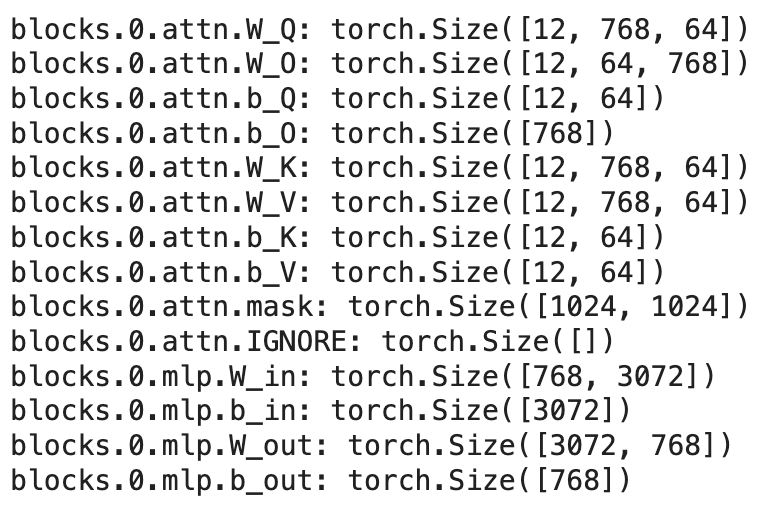
\includegraphics[width=4cm]{img/block_zero_shape.png}
    \caption*{Parameter shapes (alternate notation)}
    \label{fig:enter-label}
\end{figure}
\footnotesize
\begin{align*}
    &H = 12 \;\text{(\# heads)} \\
    % should make notation consistent
    &M = 768 \;\text{(embedding dimension)} \\
    &D = 64 \; \text{ (attention dimension)} \\
    &Z = 3072 \; \text{ (MLP dimension) }  
\end{align*}
\end{column}
\end{columns}
\end{frame}

\begin{frame}{Multiheaded attention}
\footnotesize
\begin{align*}
A_b (x) &= O_b^L ((s^{HL_2} ( \frac{ (Q_b^L(x))_{d}  (K_b^L(x))^d}{\sqrt{D}} ))^D_{l_1} (V_{b}^L (x))^l)
\end{align*}
\begin{columns}
\begin{column}{.5\textwidth}
\begin{itemize}
\item Einstein notation ($c_i x^i = \sum_{i} c_i x_i$)
\item Can use two values of $D$ (i.e. $D_{VO}, D_{QK}$)
\item $l_1, l_2$ two axes of {\it attention matrix} $s^{HL_2} ( \frac{ (Q_b^L(x))_{d}  (K_b^L(x))^d}{\sqrt{D}} )$
\end{itemize}
\begin{figure}
    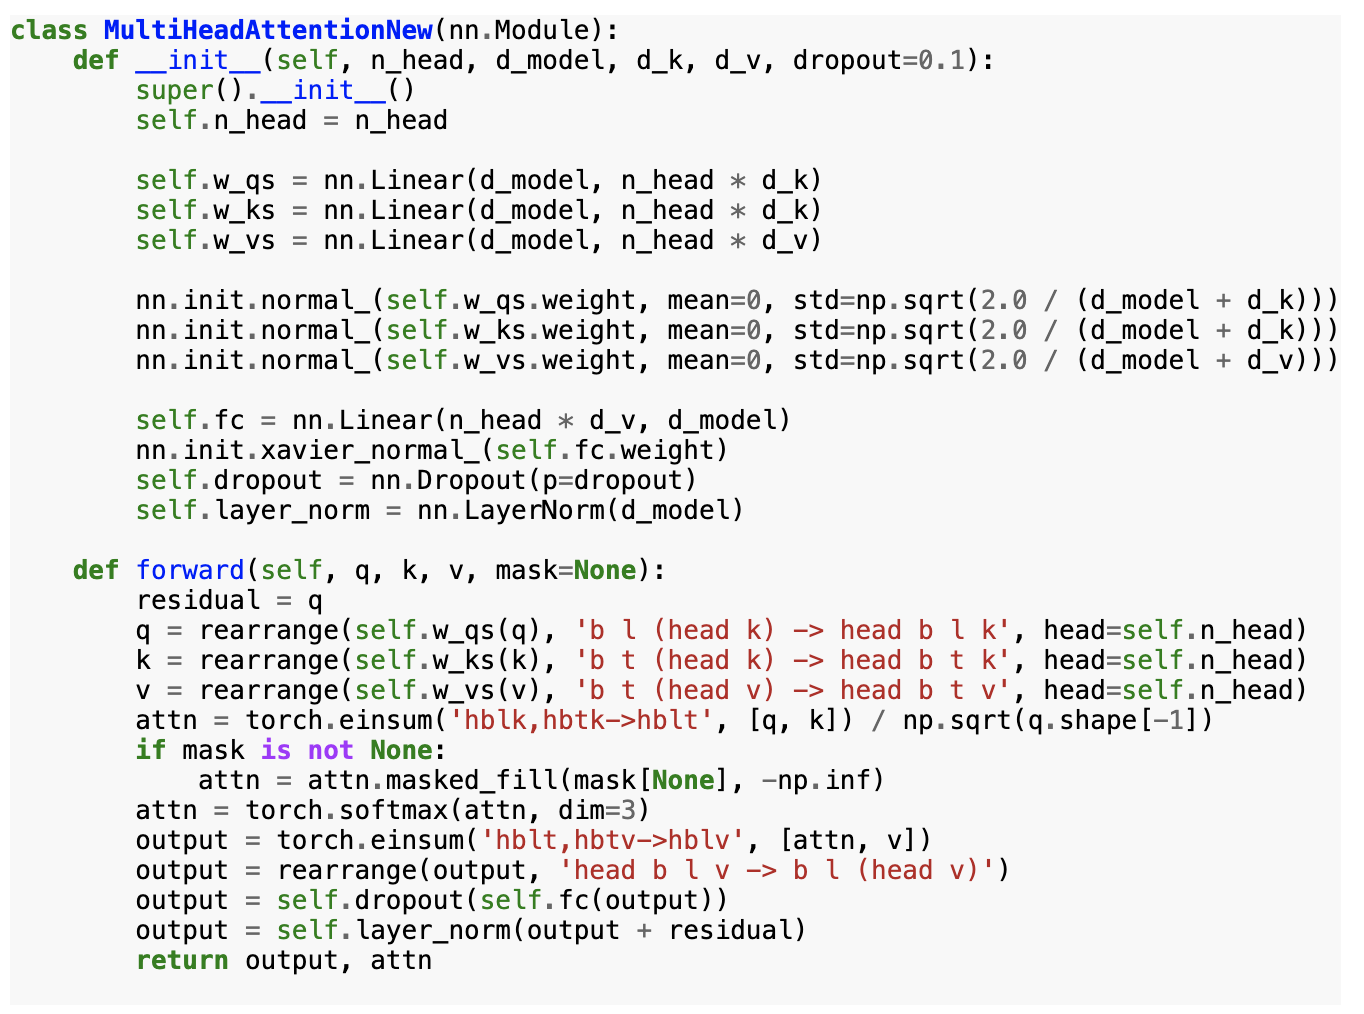
\includegraphics[width=4cm]{img/multihead.png}
    \caption*{\citet{einops-undated-sp}}
\end{figure}
\end{column}
\begin{column}{.5\textwidth}
\tiny
\vspace{-1cm}
\begin{align*}
\text{ softmax } s : \mathbb R^{L } &\to \mathbb R^{L } \\
\hline
Q_b: \mathbb R^{M \times H} &\to \mathbb R^{D \times H} \\
x &\mapsto (W_{Q_b})_{m} x^{m} \\ 
W_{Q_b} &\in \mathbb R^{M \times D \times H} \\
\hline
K_b: \mathbb R^{M \times H} &\to \mathbb R^{D  \times H} \\
x &\mapsto (W_{K_b})_{m} x^{m} \\ 
W_{K_b} &\in \mathbb R^{M \times D \times H}\\
\hline
V_b: \mathbb R^{M  \times H} &\to \mathbb R^{D   \times H} \\
x &\mapsto (W_{V_b})_{m} x^{m} \\ 
W_{V_b} &\in \mathbb R^{M \times D \times H} \\
\hline
O_b: \mathbb R^{D \times H} &\to \mathbb R^{M} \\
x &\mapsto (W_{O_b})_{hd} x^{hd} \\ 
W_{O_b} &\in \mathbb R^{M \times D \times H} 
\end{align*}
\end{column}
\end{columns}
\end{frame}

\begin{frame}{Multilayer perceptron (MLP)}
\begin{itemize}
    \item Transformers traditionally use two layer MLP
\end{itemize}
    \begin{align}
        M_b = 
    \end{align}
\end{frame}

\begin{frame}{Residual stream}

We may think of computation up to each block as an iteratively refined projection $\tilde T_l: \mathcal H^L \to \mathbb R^{m \times L}$
\begin{columns}
\begin{column}{.5\textwidth}
\begin{itemize}
    \item The attention dimension $D$ constrains the subspace of the residual stream operated on by each component (i.e. $D < M$.
    \item The output of each block is added to the input and fed to the next block
    \item Thus, we call the state of the $L$ tokens in the $m$ dimensional embedding space the {\it residual stream.}
    \item The dimension of $W_O$ and $W_I$ is lower than the residual stream, so blocks may edit it orthogonally.
\end{itemize}
\end{column}
\begin{column}{.5\textwidth}
\begin{figure}
    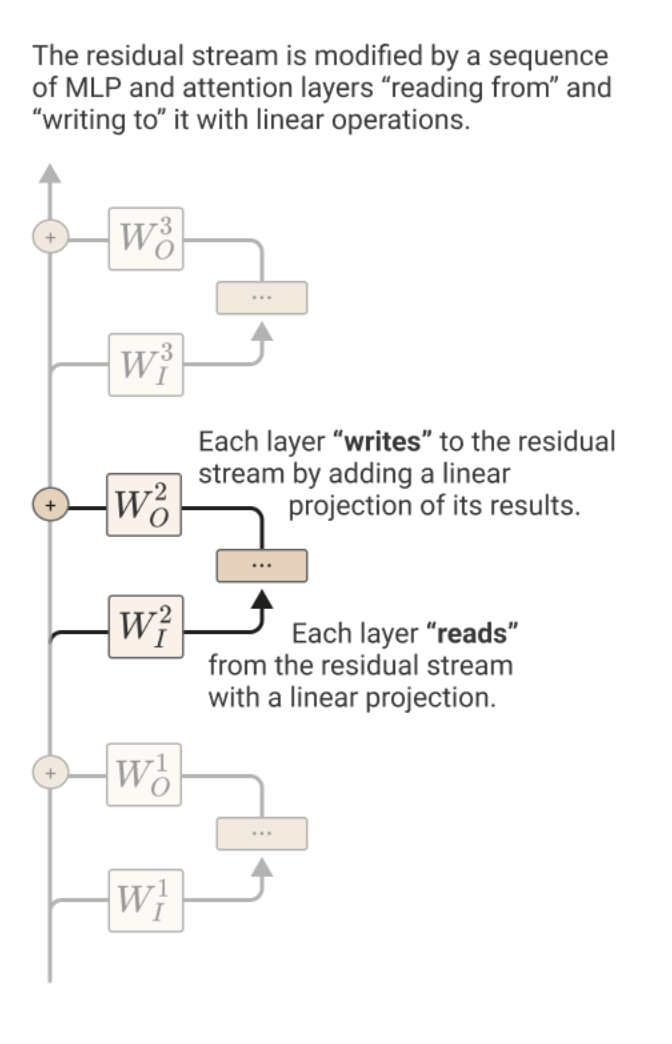
\includegraphics[width = 3cm]{img/transblock.png}
    \caption*{Structure across blocks \citep{Nanda-wv}}
\end{figure}
\end{column}
\end{columns}
\end{frame}


% \begin{frame}{Attention}
%     \begin{algorithmic}
% \tiny
% \Function{Attention}{$Q, K, V$}
%     \State $A \gets \text{softmax}\left(\frac{QK^T}{\sqrt{d_k}}\right)V$
%     \State \textbf{return} $A$
% \EndFunction
% \end{algorithmic}
% \end{frame}

% \begin{frame}{Multi-headed Attention}
%     \begin{algorithmic}
% \tiny
% \Function{MultiHeadAttention}{$X, W_h^Q, W_h^K, W_h^V$}
%     \For{$h = 1, \dots, H$}
%         \State $Q_h \gets XW_h^Q$
%         \State $K_h \gets XW_h^K$
%         \State $V_h \gets XW_h^V$
%         \State $\text{head}_h \gets \Call{Attention}{Q_h, K_h, V_h}$
%     \EndFor
%     \State \textbf{return} $\text{Concat}(\text{head}_1, \dots, \text{head}_H)W^O$
% \EndFunction
% \end{algorithmic}
% \end{frame}

% \begin{frame}{MLP-layer}
% \begin{algorithmic}
% \tiny
% \Function{FeedForward}{$x$}
%     \State $x \gets \text{max}(0, xW_1 + b_1)W_2 + b_2$
%     \State \textbf{return} $x$
% \EndFunction
% \end{algorithmic}
% \end{frame}

% \begin{frame}{Structure of transformer block}
% \begin{algorithmic}
% \tiny
% \Function{Transformer Block}{$X$}
% \State \textbf{Input:} $X \in \mathbb{R}^{N \times D}$  \Comment{Input matrix of sequence embeddings}
% \State \textbf{Output:} $\text{Output} \in \mathbb{R}^{N \times D}$ \Comment{Transformed sequence}
% \State \textbf{Parameters:}
% \State $W^Q, W^K, W^V \in \mathbb{R}^{D \times d_k}$ \Comment{Projection matrices for Q, K, V}
% \State $W^O \in \mathbb{R}^{D \times D}$ \Comment{Output projection matrix}
% \State $W_1 \in \mathbb{R}^{D \times d_{ff}}, W_2 \in \mathbb{R}^{d_{ff} \times D}$ \Comment{FFN weights}
% \State $b_1, b_2 \in \mathbb{R}^{d_{ff}}$ \Comment{FFN biases}

%     \State $Z \gets \text{LayerNorm}(X + \Call{MultiHeadAttention}{X})$ \Comment{Apply attention}
%     \State $\text{Output} \gets \text{LayerNorm}(Z + \Call{FeedForward}{Z})$ \Comment{Apply FFN}
%     \State \textbf{return} $\text{Output}$
%     \EndFunction
% \end{algorithmic}

% \end{frame}

% \begin{frame}{Training a sequential transformer}

% \end{frame}

% \begin{frame}{Inference a sequential transformer}
% Caveat: "Inference = prediction" in AI, "inference = estimation" in statistics
% \end{frame}


% \begin{frame}
% Problems with large dictionaries:
% \begin{itemize}
%     \item Overcompleteness: multiple valid solutions \cite{Scott_Shaobing_Chen_David_L_Donoho_Michael_A_Saunders2001-hh}
% \end{itemize}
% \end{frame}
